\documentclass{article}
\usepackage[utf8]{inputenc}
\usepackage{graphicx}
\usepackage[
backend=biber,
style=authoryear,
citestyle=authoryear
]{biblatex}
\renewcommand*{\bibfont}{\small}
\usepackage[normalem]{ulem}
\usepackage{fancyhdr}
\usepackage{multicol}
\usepackage[hidelinks]{hyperref}
 
\pagestyle{fancy}
\fancyhf{}
\rhead{Can Meaning Travel?}
\lhead{Nicolai Berk}
\cfoot{\thepage}

\useunder{\uline}{\ul}{}

\addbibresource{PhD-Proposal.bib}


\usepackage{xcolor}

\title{Can Meaning Travel? The Causal Effect of Media Frames on Issue Definitions and Attitudes}
\author{Nicolai Berk\footnote{Doctoral Candidate, Dynamics Doctoral Program, Humboldt-Universität zu Berlin, \href{mailto:nicolai.berk@hu-berlin.de}{nicolai.berk@hu-berlin.de}}}
\date{September 2021}

\begin{document}

\maketitle


\begin{abstract}
    A large body of literature debates the existence and extent of effects of media framing on consumers' issue attitudes. At the same time, mechanisms of opinion formation have mainly been studied experimentally. Combining panel data from the German Longitudinal Election Study with fine-grained analyses of media framing, I address both debates with observational data. I provide evidence from 1,056 fixed-effect, difference-in-differences models suggesting systematic differences in newspaper readers' opinion shifts. Second, I show that such changes in consumers' attitudes do \textit{not} correspond to changes in the issue framing of the consumed media outlet. Instead, these changes could be explained by an ideological readership reacting differently to changes in the news agenda. Lastly, the study explores whether such changes in media framing affect consumers' issue definitions using state-of-the-art text analysis methods. The findings contribute to our understanding of opinion formation processes and the relevance of the news media in the 21st century.
\end{abstract}


\section{Introduction}

\begin{itemize}
  \item starting point: historical discussion on minimal vs maximal media effects and the discussion on external validity
  \item agenda setting yes (cite), but what about framing? Debate goes on
  \item second: unclear mechanisms - look for lab evidence to cite on this
\end{itemize}


\section{Framing in the wild}

\subsection{General evidence of framing effects}

argument 1: key issue is not the external validity of framing experiments, but more likely to observe framing effects when consuming the SAME newspaper, which one trusts already - basically cue taking (Foos, Spirig, Ladd vs Gentzkow, Guess, resolved by Slothuus and Leeper)


\subsection{Mechanisms of framing}

argument 2: opinion shifts come about through changing associations (framing/issue definition) $\rightarrow$ value expectancy framework, but with a neurological basis


\subsection{Implications for the study of framing effects}

\begin{itemize}
\item Lesson: more observational data necessary, but we need to study cases where the slant of a newspaper that people already read changes, without obvious changes eg in ownership that made readers discount the slant
\item people could a) not react, b) stop reading their newspaper, c) change their opinion
\item changes in issue association (in the news) should affect people's issue definitions, which changes their opinion on the issue.
\end{itemize}


\section{Study design}

\subsection{Data and case description}

\subsubsection{Public opinion data}

% plot with opinion development per paper for four / six issues

\begin{itemize}
    \item GLES Panel 2016-2020
    \item about 10,000 - 15,000 respondents per wave
    \item data on issue attitudes, importance, and news consumption
\end{itemize}

\begin{figure}[!ht]
    \centering
    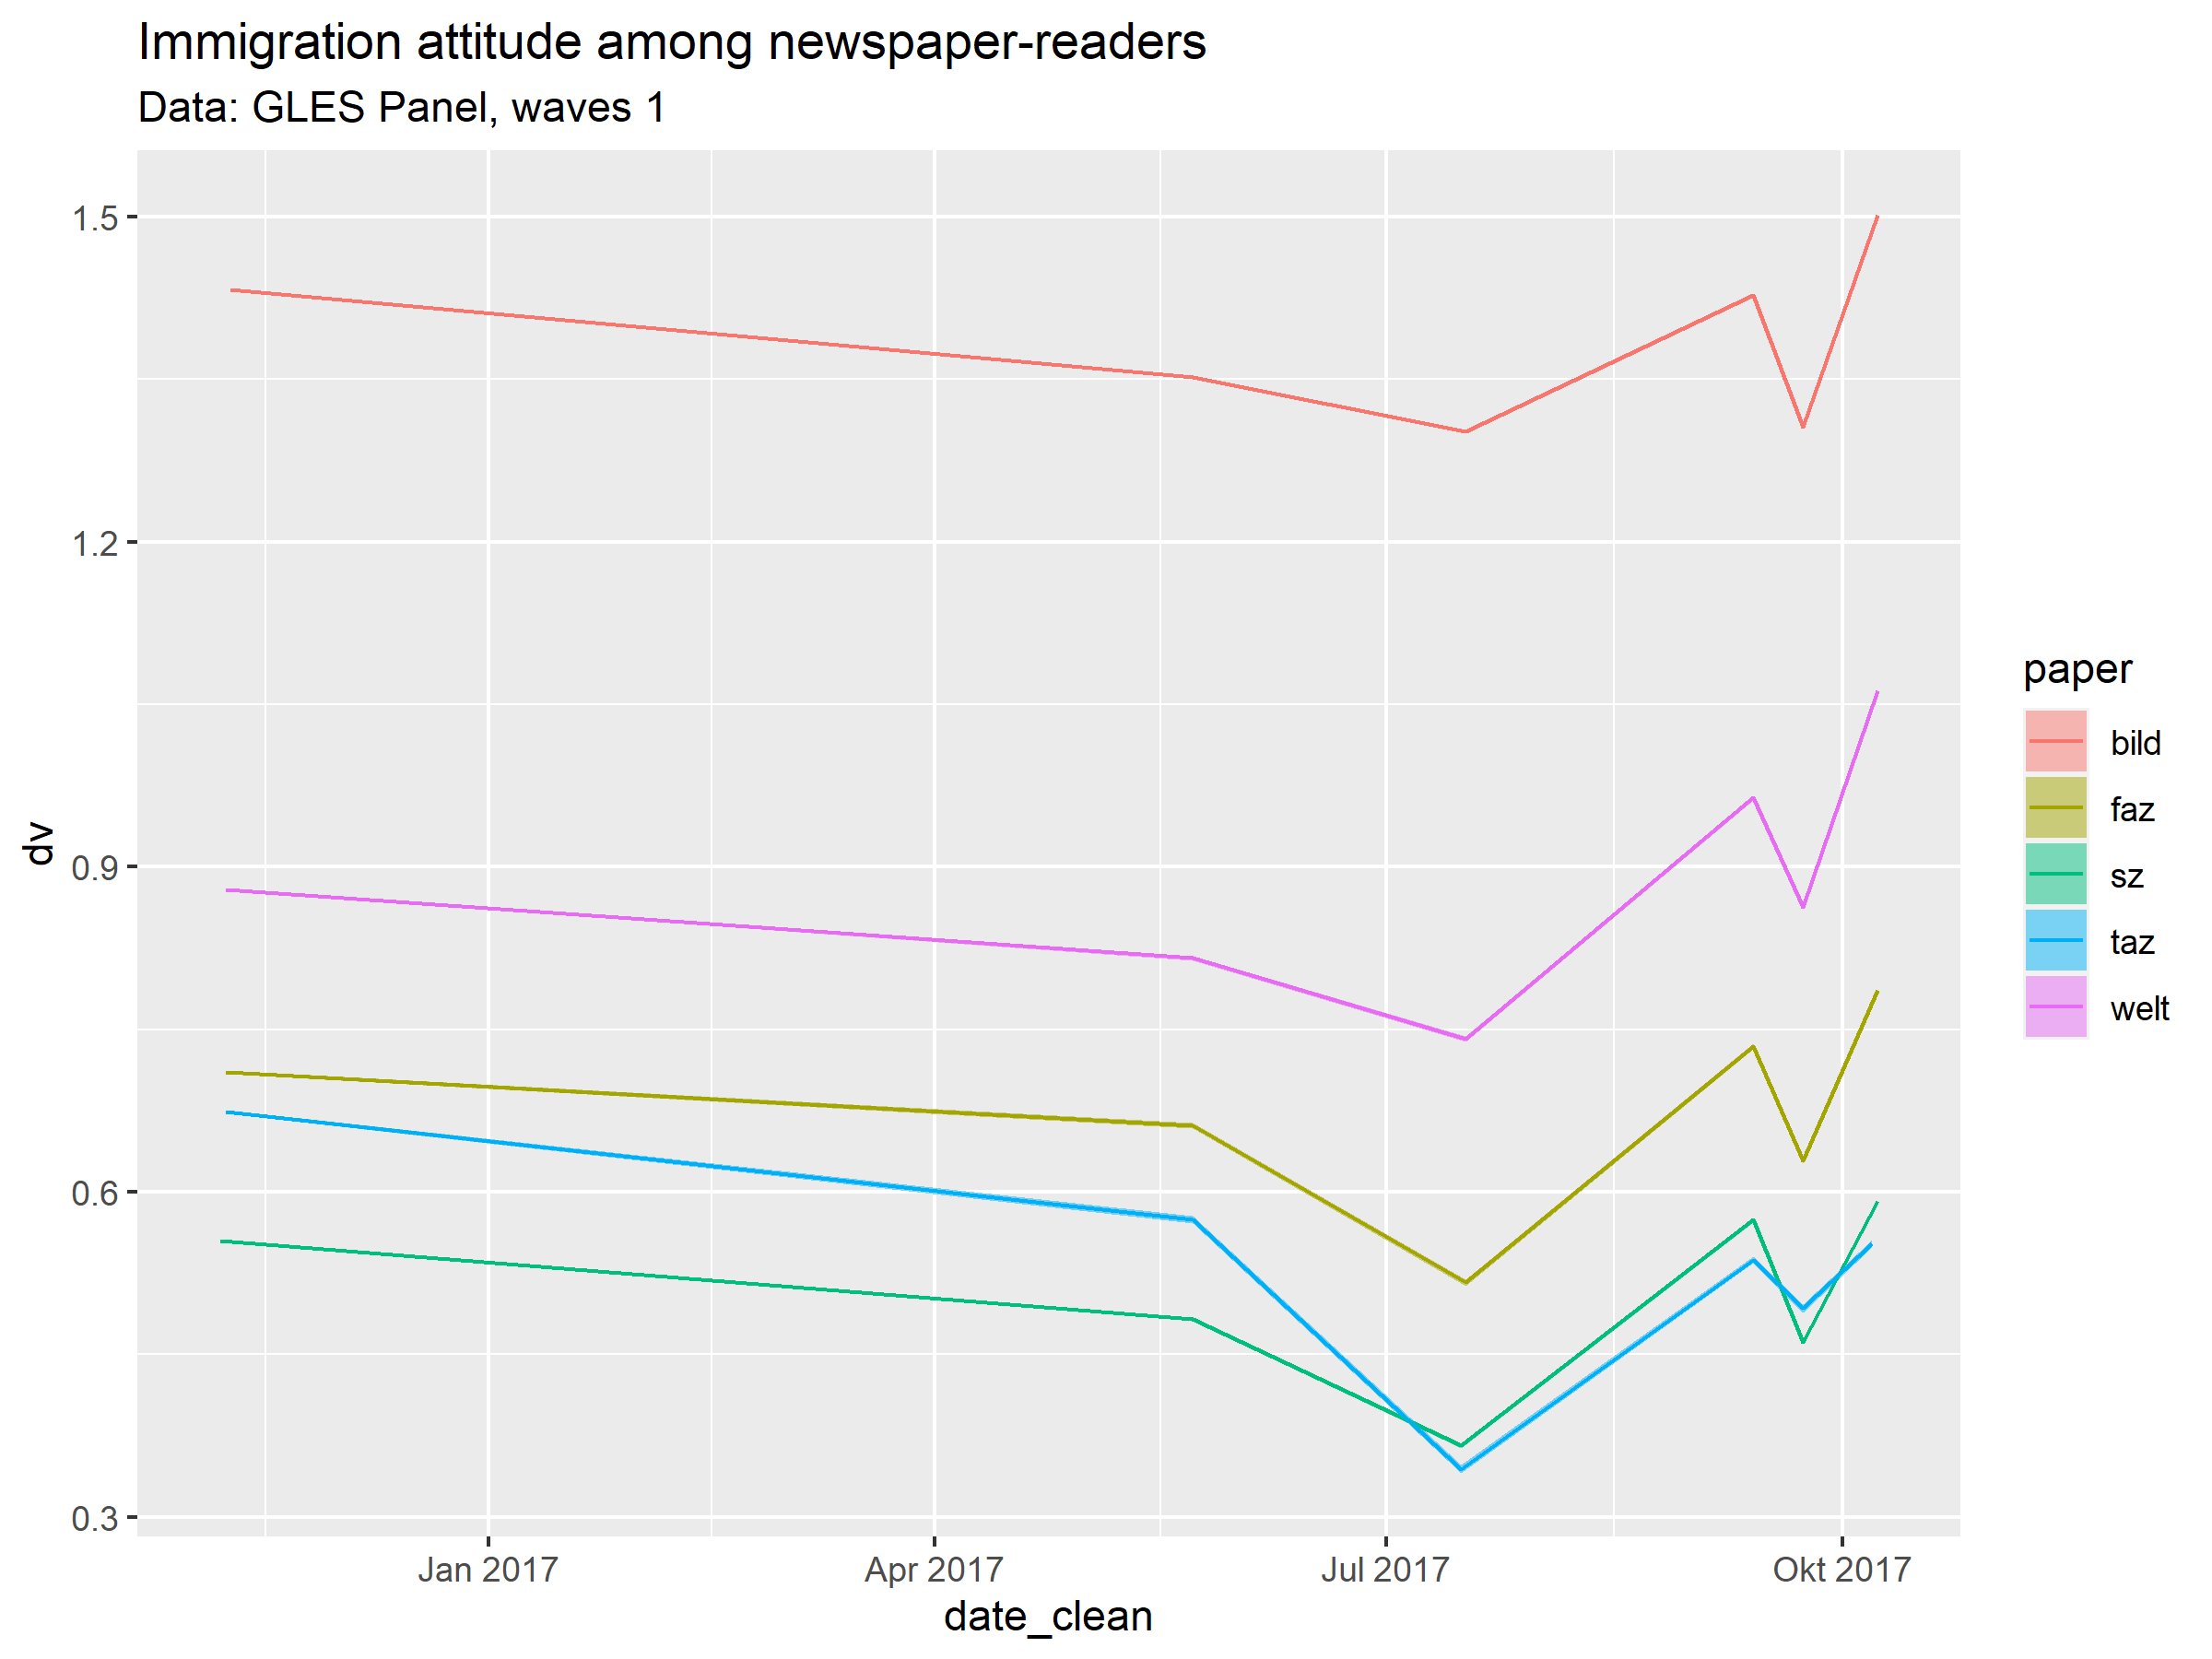
\includegraphics[width=\textwidth]{paper/vis/Immigration_papers.png}
    \caption{Opinions on migration across time (higher values indicate more restrictive attitudes).}
    \label{fig:issues}
\end{figure}


\subsubsection{Data on news framing}
% plot with frames and survey dates
\begin{figure}[!ht]
    \centering
    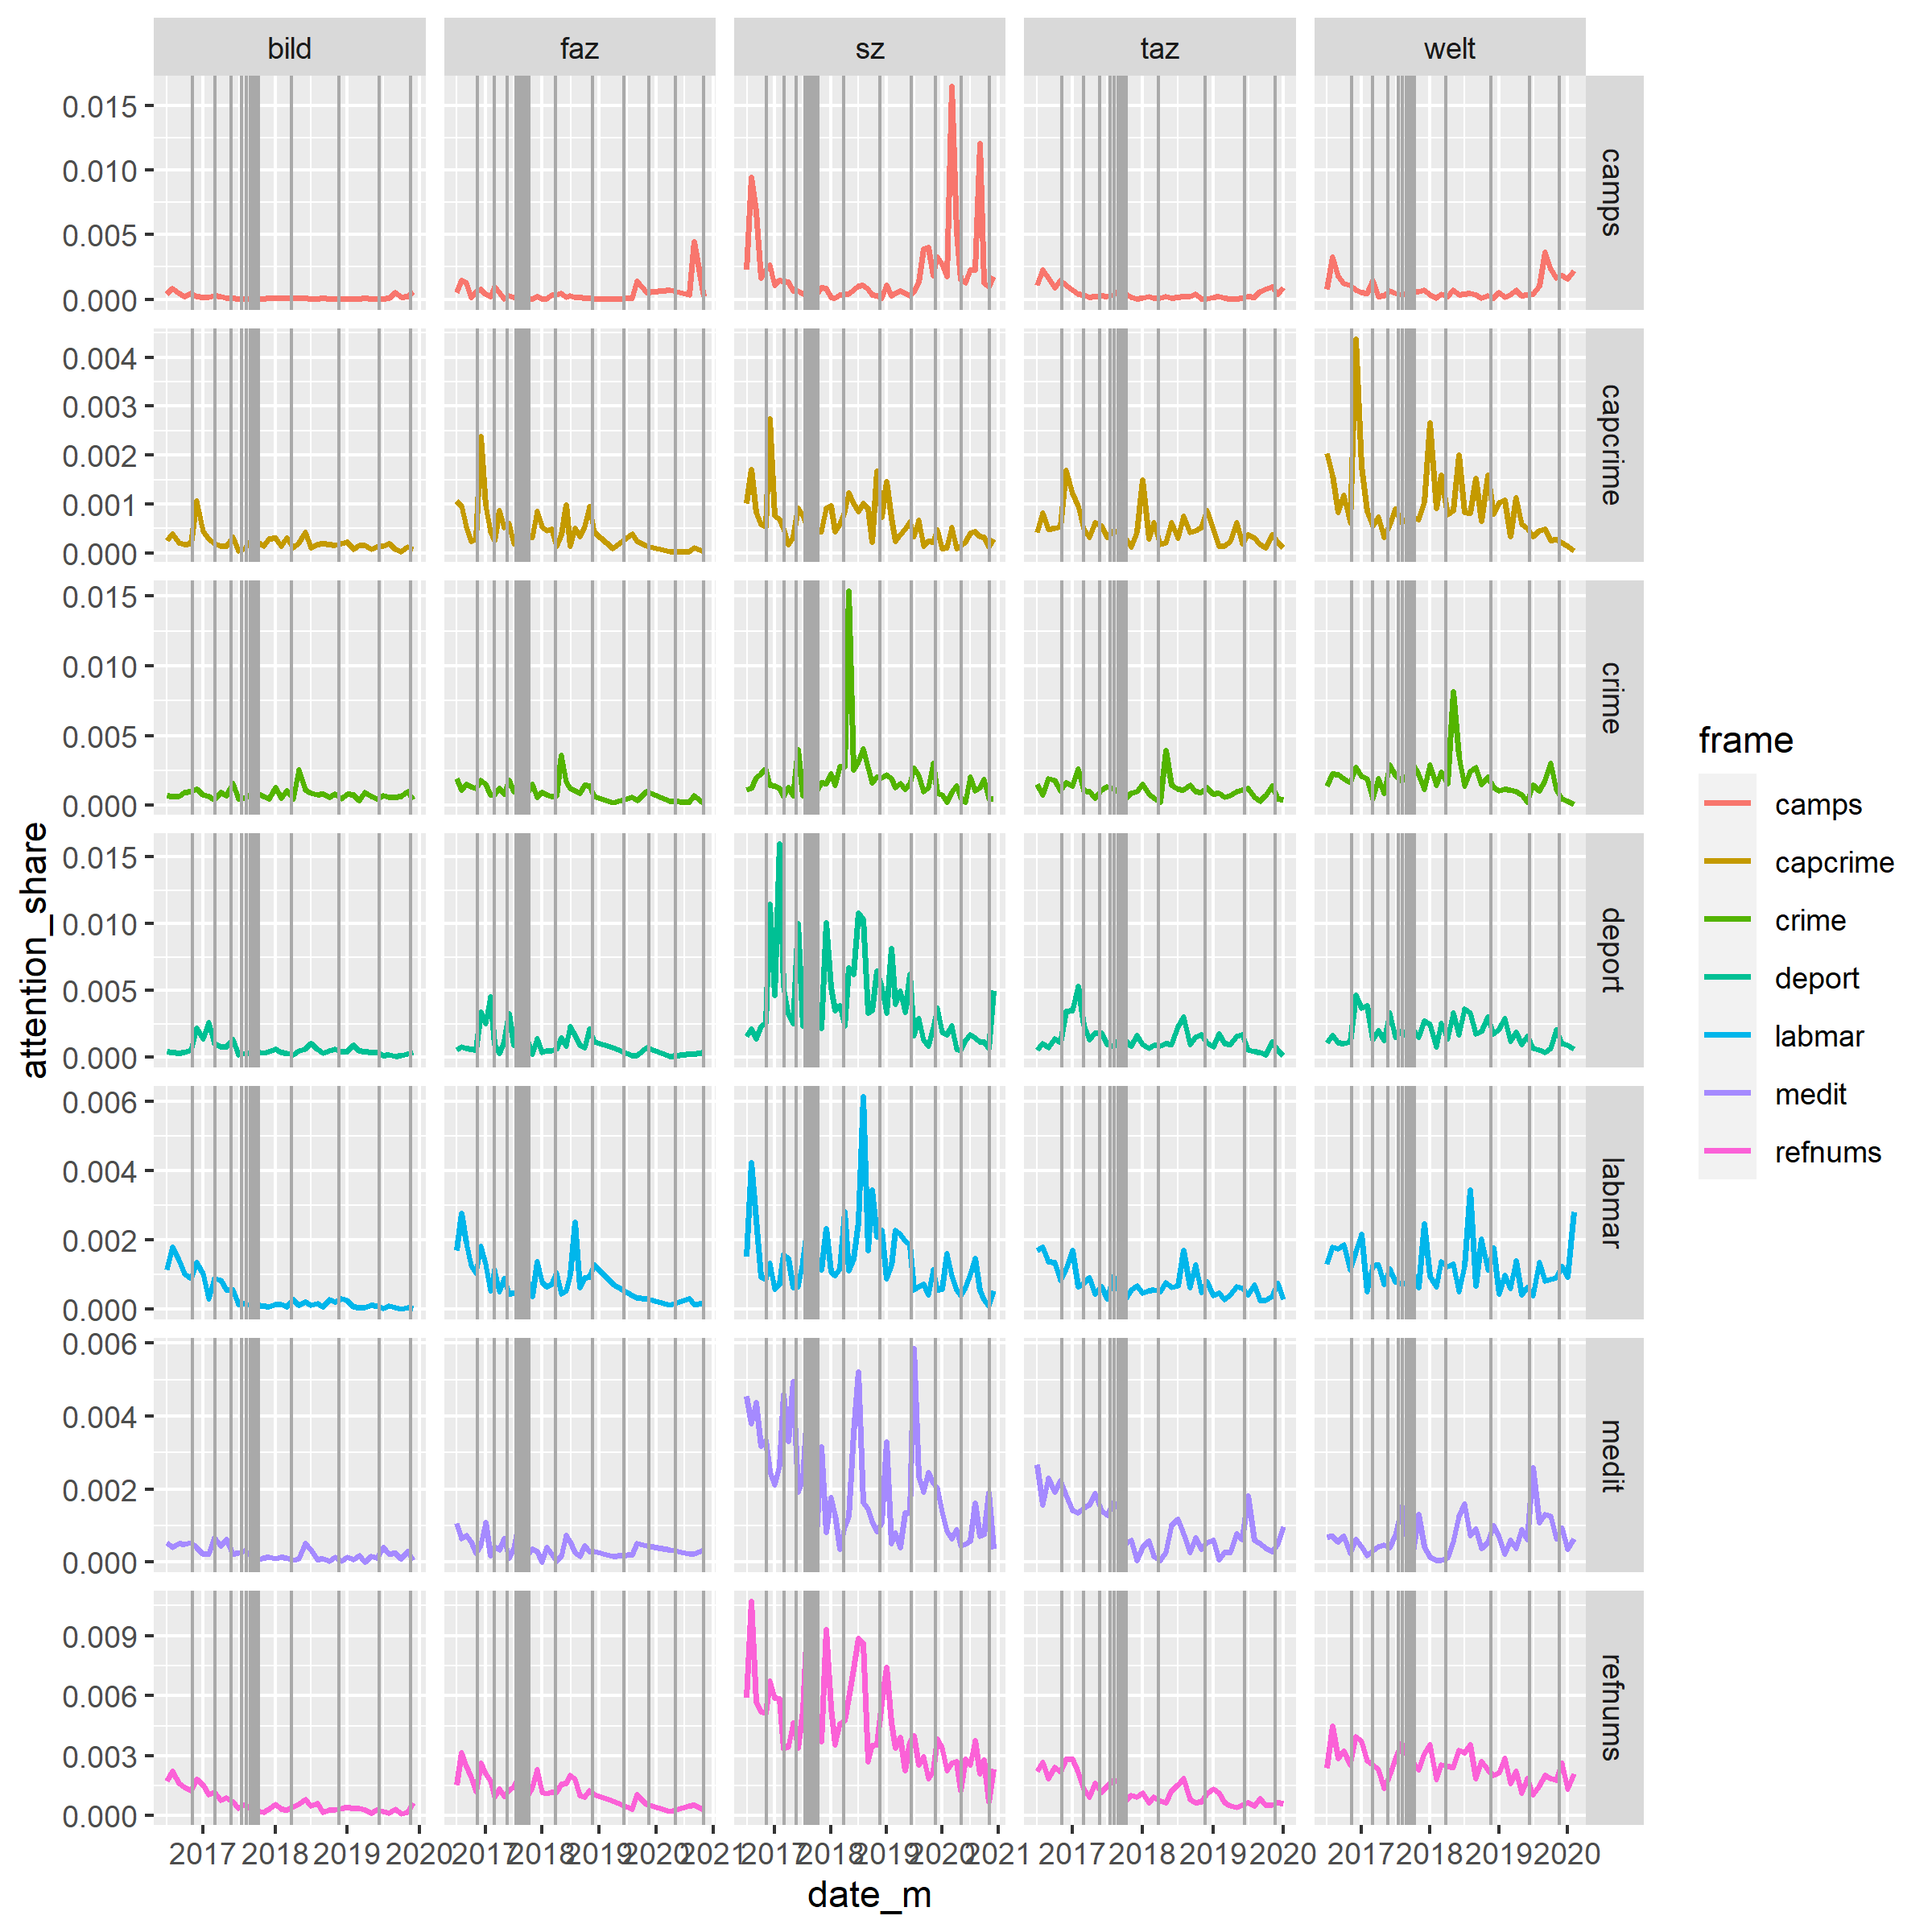
\includegraphics[width=\textwidth]{paper/vis/frames_papers_wtd_focus.png}
    \caption{Prevalence of different migration frames across newspapers. Gray vertical lines indicate survey field dates.}
    \label{fig:frames}
\end{figure}

\begin{itemize}
    \item Collected around 2.5 million newspaper articles from six major newspapers
    \item Extracted and annotated a stratified sample of articles using a migration dictionary
    \item Trained a migration classifier (BERT transformer) based on these annotations
    \item estimated migration frames using STM on migration articles only (N = 90,000): 
    \item retained most common and relevant frames that allow to form clear hypotheses about attitude formation:
    \begin{itemize}
        \item Internment camps, 
        \item capital crime (sexual assault/rape/murder) committed by refugees, 
        \item general petty crime by refugees and issues in refugee living quarters in Germany,
        \item deportations,
        \item labour market needs for and integration of refugees
        \item drownings in the mediterranean
        \item refugee numbers
    \end{itemize}
\end{itemize}



\subsection{Study design}

\subsubsection{Can framing effects among newspaper readers be observed?}

To get a glimpse of whether opinion shifts might be influenced by news consumption, I estimate difference-in-differences models (DiDs) for all available combinations of news outlets (incl. TV news), issues, and survey waves. The main term of interest is the interaction of a binary indicator of readership of a certain outlet with a binary indicator which equals 1 for the current wave and 0 for the preceding wave. That means I measure the shift in opinions of the readership of a certain outlet, controlling for the changes taking place among consumers of other news.

\subsubsection{Can these opinion shifts be explained by changing media frames?}

\begin{itemize}
    \item look at migration, maybe a second issue: how strongly do DiD's correlate with changing frame prevalence/DiD of frame attention?
    \item look at how FE model DiD's change when controlling for newspaper attention/DiD
    \item add right-wing slant as second dependent using AfD-classifier
\end{itemize}

\subsubsection{Have readers' issue definitions changed as a result of the changing media frames?}

The final analysis in this paper aims to show that changes in readers' migration definitions correspond to changes in news coverage. This can be achieved by applying embedding regression to open survey responses, which shows differing word associations for subgroups of documents. This would show if respondents reading a certain newspaper define migration more in line with e.g. the humanitarian situation in refugee camps, compared to a preceding wave and controlling for shifts in other newspapers.

\section{Results}

\subsection{DiD-assumption: Parallel trends}

% refer to graph on mig issue
The parallel trends assumption is met, as can be seen in figure \ref{fig:issues}. A plot of all other issues showing similar co-variation will be added to the appendix at a later point in time.
    
% also think about excludability: how can you ensure that these shifts are a result of media framing (this might be answered in number two)

\subsection{Distribution of DiD-effect significance}

The upper panel of figure \ref{fig:p_values} shows the distribution of p-values for the DiD-term from 1,056 fixed-effect models with GLES Panel data. The distribution shows a considerable deviation from the expected uniform distribution (visible in the lower panel) were there no explaining variation in the DiD-term beyond the uniform effects of wave and paper readership. This means, more often than random, the opinions of consumers of certain news deviate from the opinions of other citizens.

% show distribution of p-values vs theoretical distribution -> looks like there is systematic deviation
\begin{figure}[!ht]
    \centering
    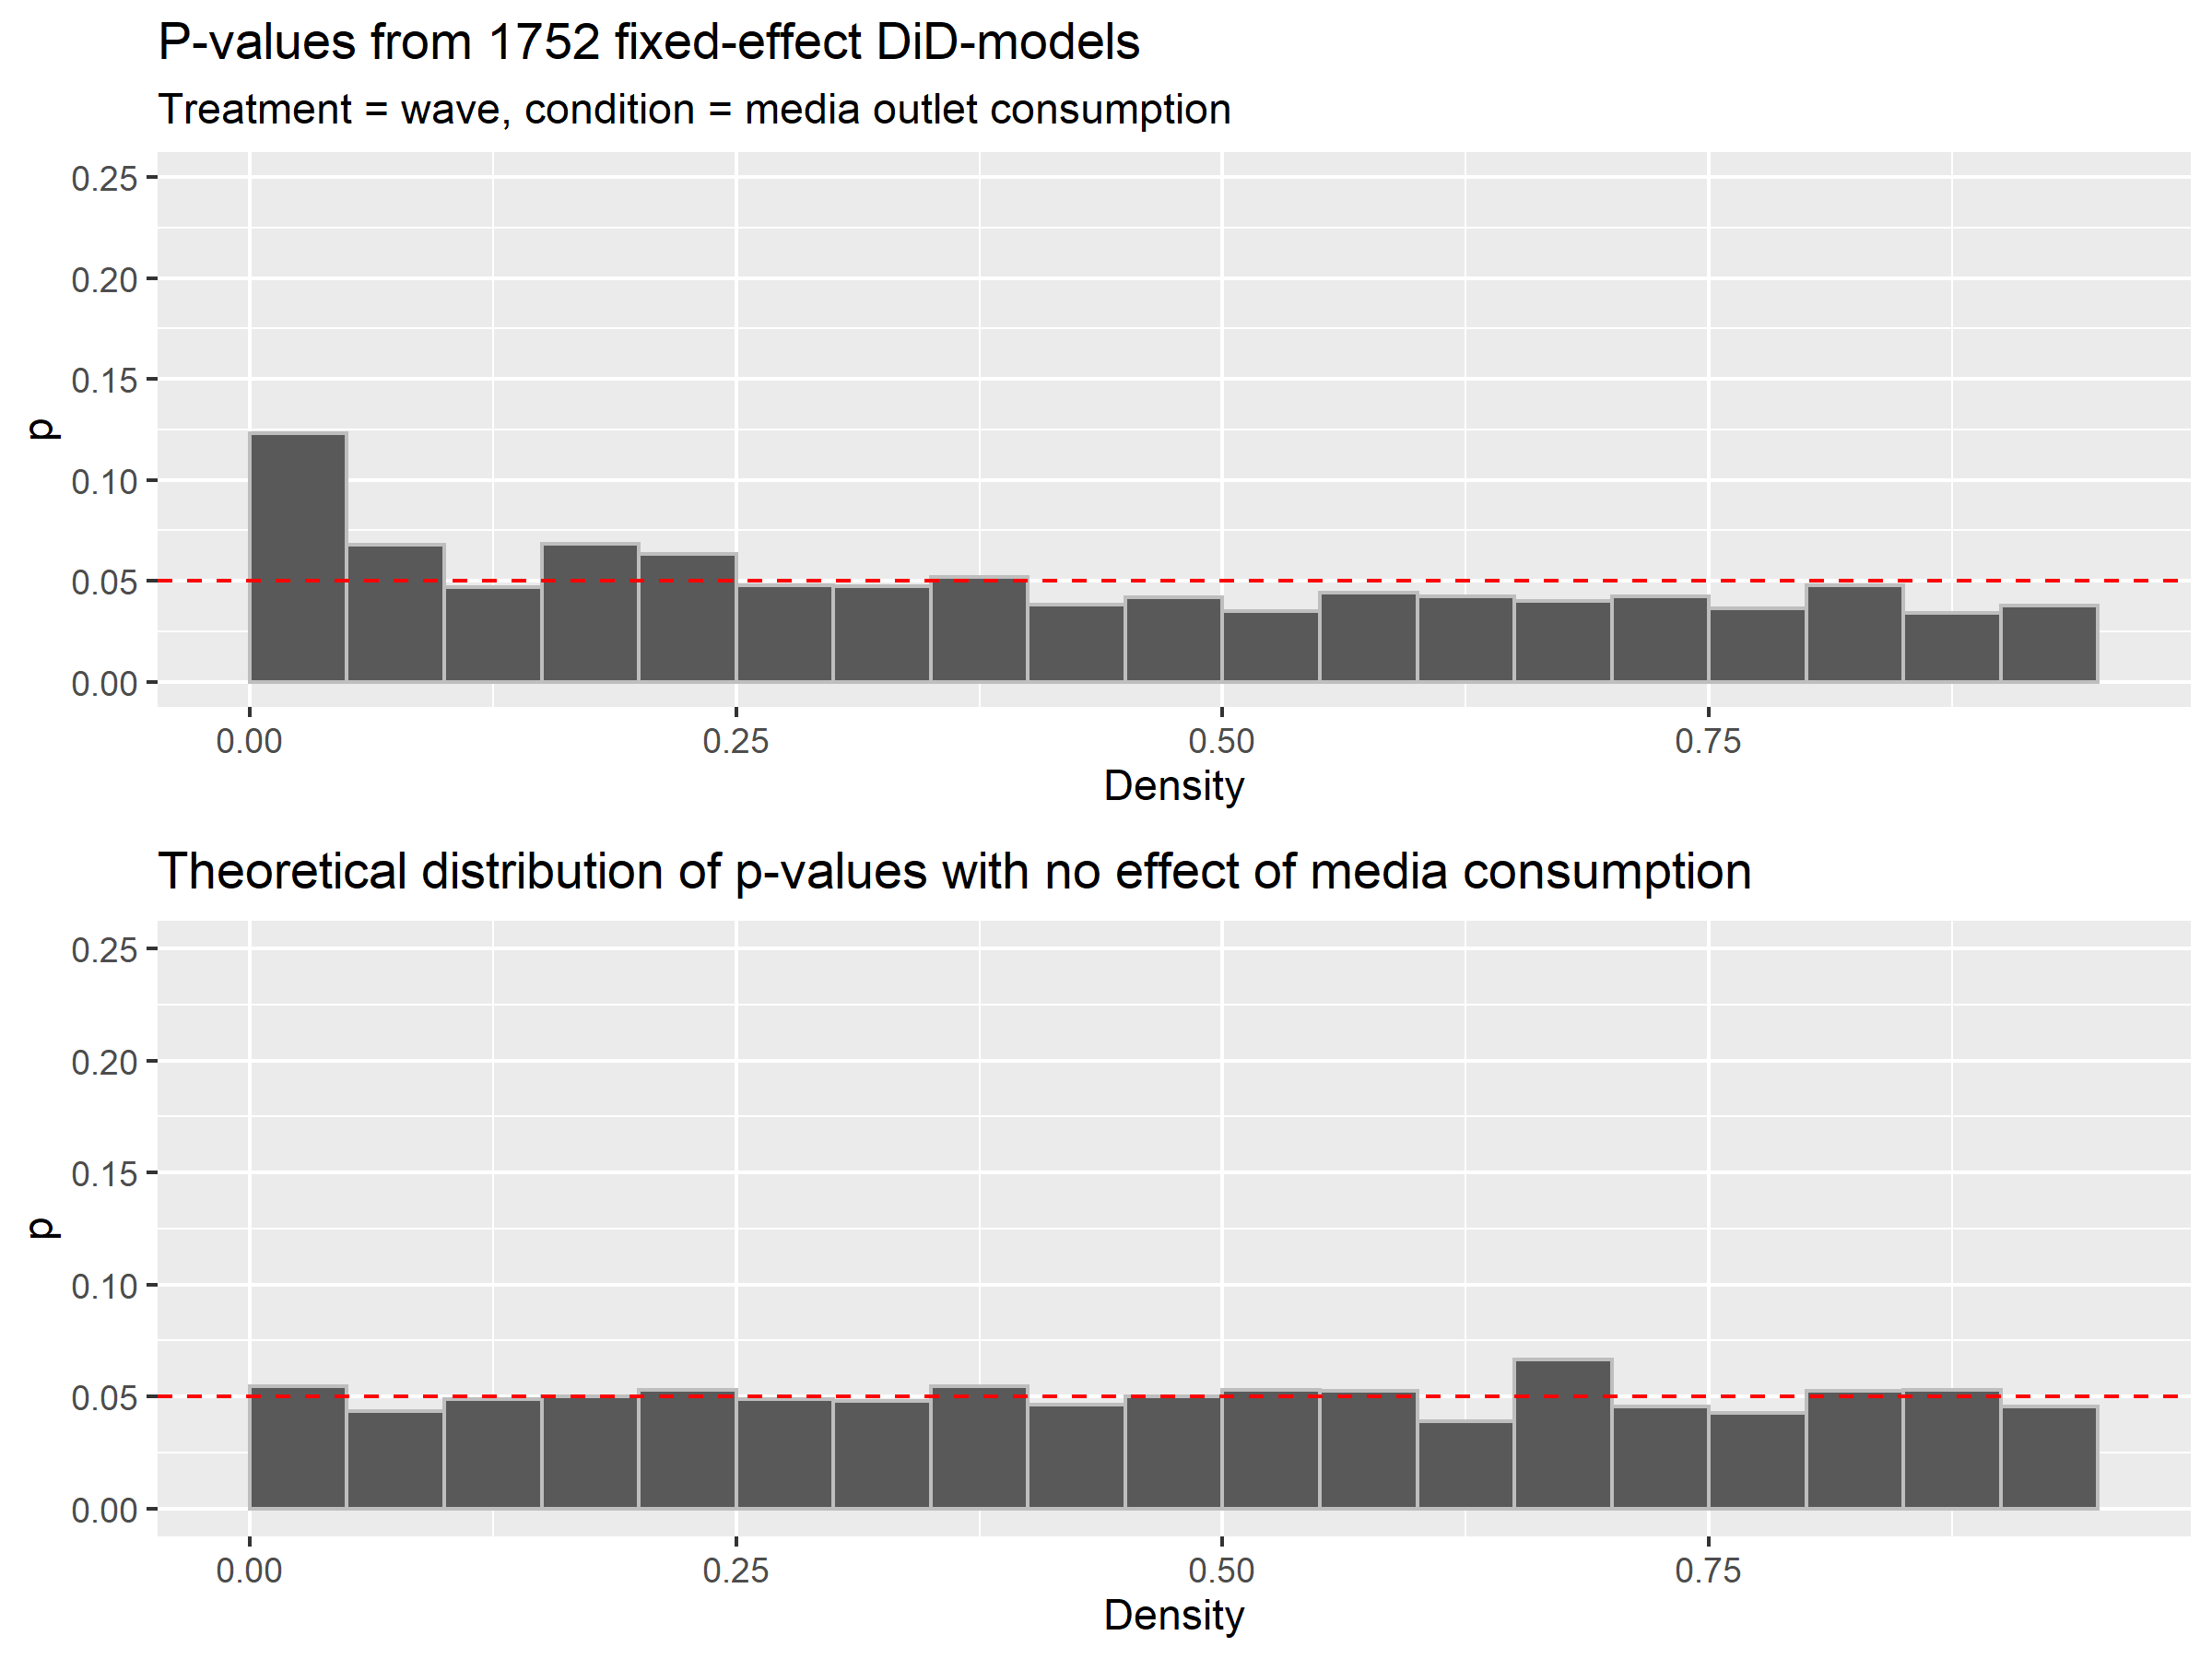
\includegraphics[width=\textwidth]{paper/vis/DiD_model_ps.png}
    \caption{Empirical and theoretical p-values of 1,363 DiD-models.}
    \label{fig:p_values}
\end{figure}



\subsection{Correlation of DiD with frame prevalence}
% show correlation of DiD with prevalence of media frames (STM)
\begin{figure}[!ht]
    \centering
    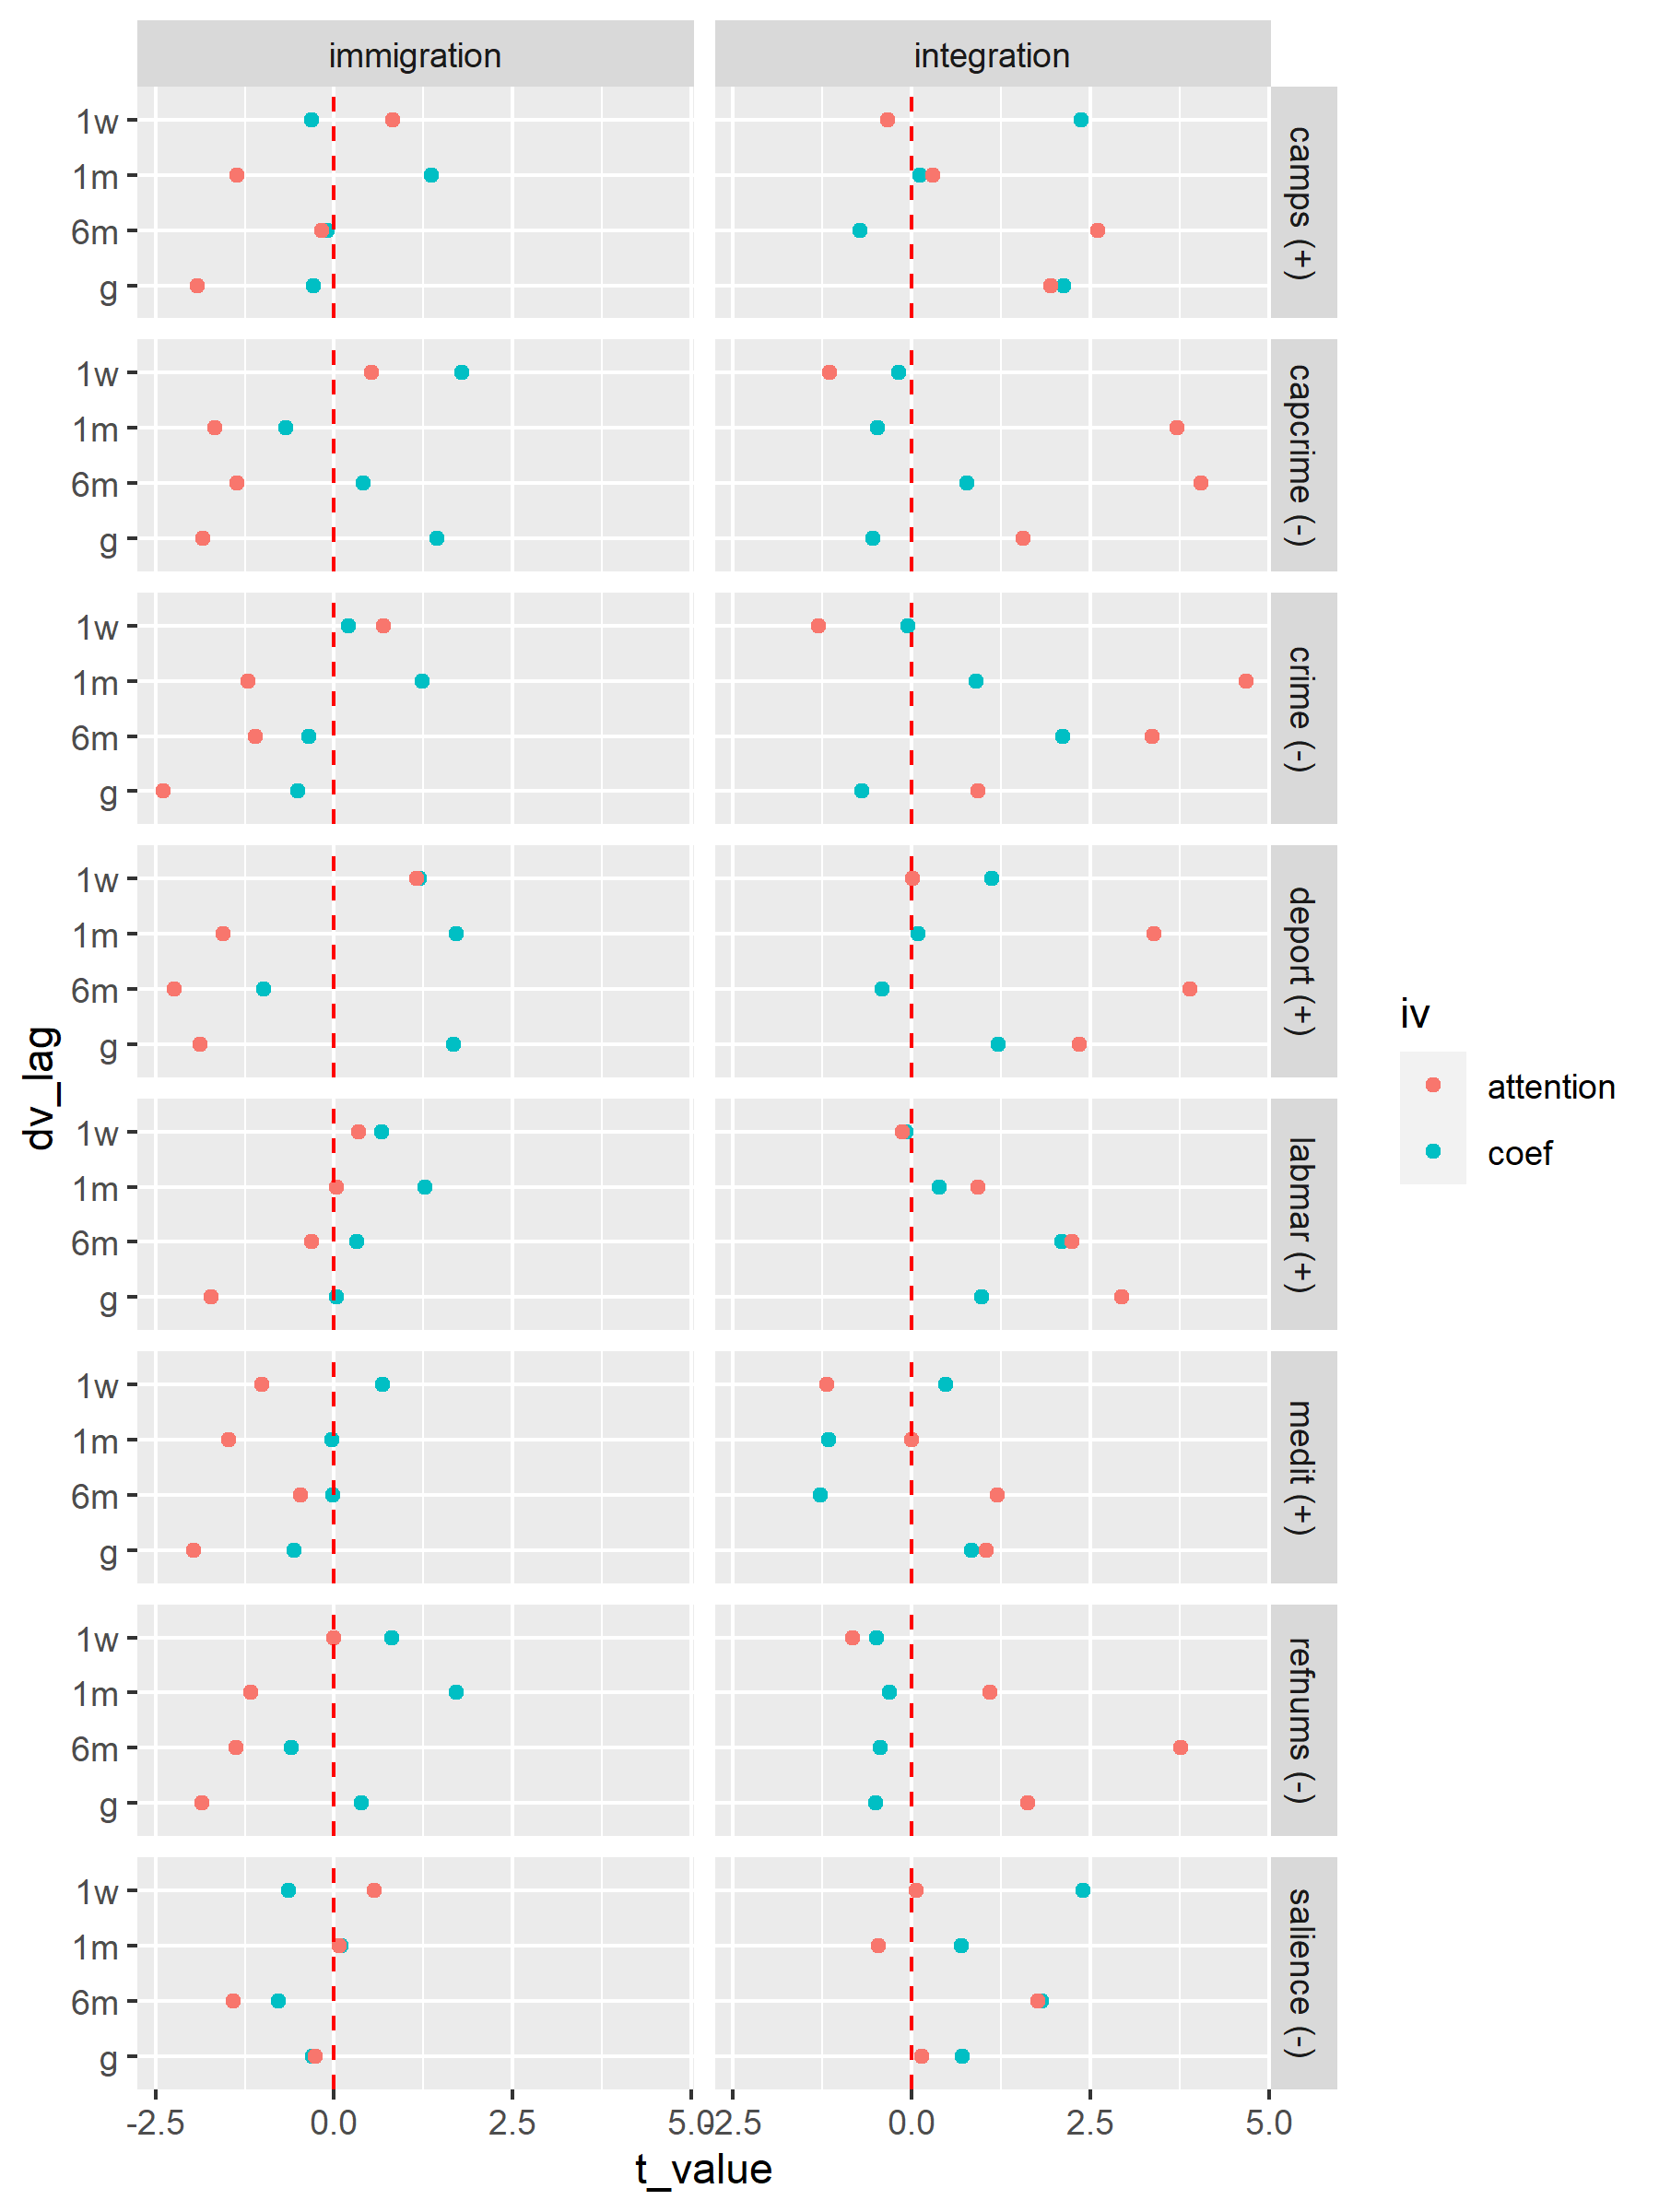
\includegraphics[width=\textwidth]{paper/vis/effectplot_noimp.png}
    \caption{Correlation of opinion shifts (DiDs) with media attention or shifts in attention (DiD's) for different specifications.}
    \label{fig:did_corr}
\end{figure}

Figure \ref{fig:did_corr} shows the core analysis to estimate the effect of media attention on reader opinion. Each dot in this graph represents the t-value of a model explaining aggregate opinion shifts (DiDs, blue dots) with aggregate media attention or shifts in attention (DiDs) for a specific frame and a specific model specification. These aggregate parameters come from models explaining immigration opinion/media attention with news outlet-wave interactions, as in the models providing the p-values for figure \ref{fig:p_values}. If opinion shifts among newpapers' readers - relative to other readers - can be explained by shifts in newspapers' issue framing, these two variables should be highly correlated. The displayed estimates are hence obtained by regressing the resulting DiD-estimates for issue attitudes on the DiD-estimates for media attention.

For example, the left graph in the top panel row shows the effect of media attention on immigration attitudes for two different independent variables (DiD \textit{coef}ficients estimating the increase in news coverage in the consumed outlet relative to all others, and the general \textit{attention} in the preceding period) and four different time lags (see horizontal lines in descending order: 1 week, 1 month, 6 months, and the full period until last survey wave [g]). Note that immigration and integration are inversely coded. Higher values indicate more restrictive attitudes on immigration, but more liberal attitudes on integration. +/- signs corresponding to the frames (visible on the right-hand side) indicate the hypothesized effect of the frame on integration.

The analysis shows that, generally, no clear pattern can be observed in the correlation of these effects. Independent of the choice of the dependent variable, specification of the independent variable (DiD/attention and differing periods of news coverage), and across all migration frames, t-values scatter around 0 (see also \ref{fig:t_values} in the appendix). This constitutes strong evidence against an effect of news framing on opinion formation. Even changes in issue salience in a given newspaper do not correspond to changes in readers' issue attitudes (see bottom two panels).

A second analysis will estimate the decrease in explanatory value of the wave-news consumption interaction/DiD when media attention is added as a control.

\subsection{Shifts in issue definitions}

% show for one specific case that shift in media frame corresponded to 

\section{Discussion}

\section{Appendix}

\begin{figure}
    \centering
    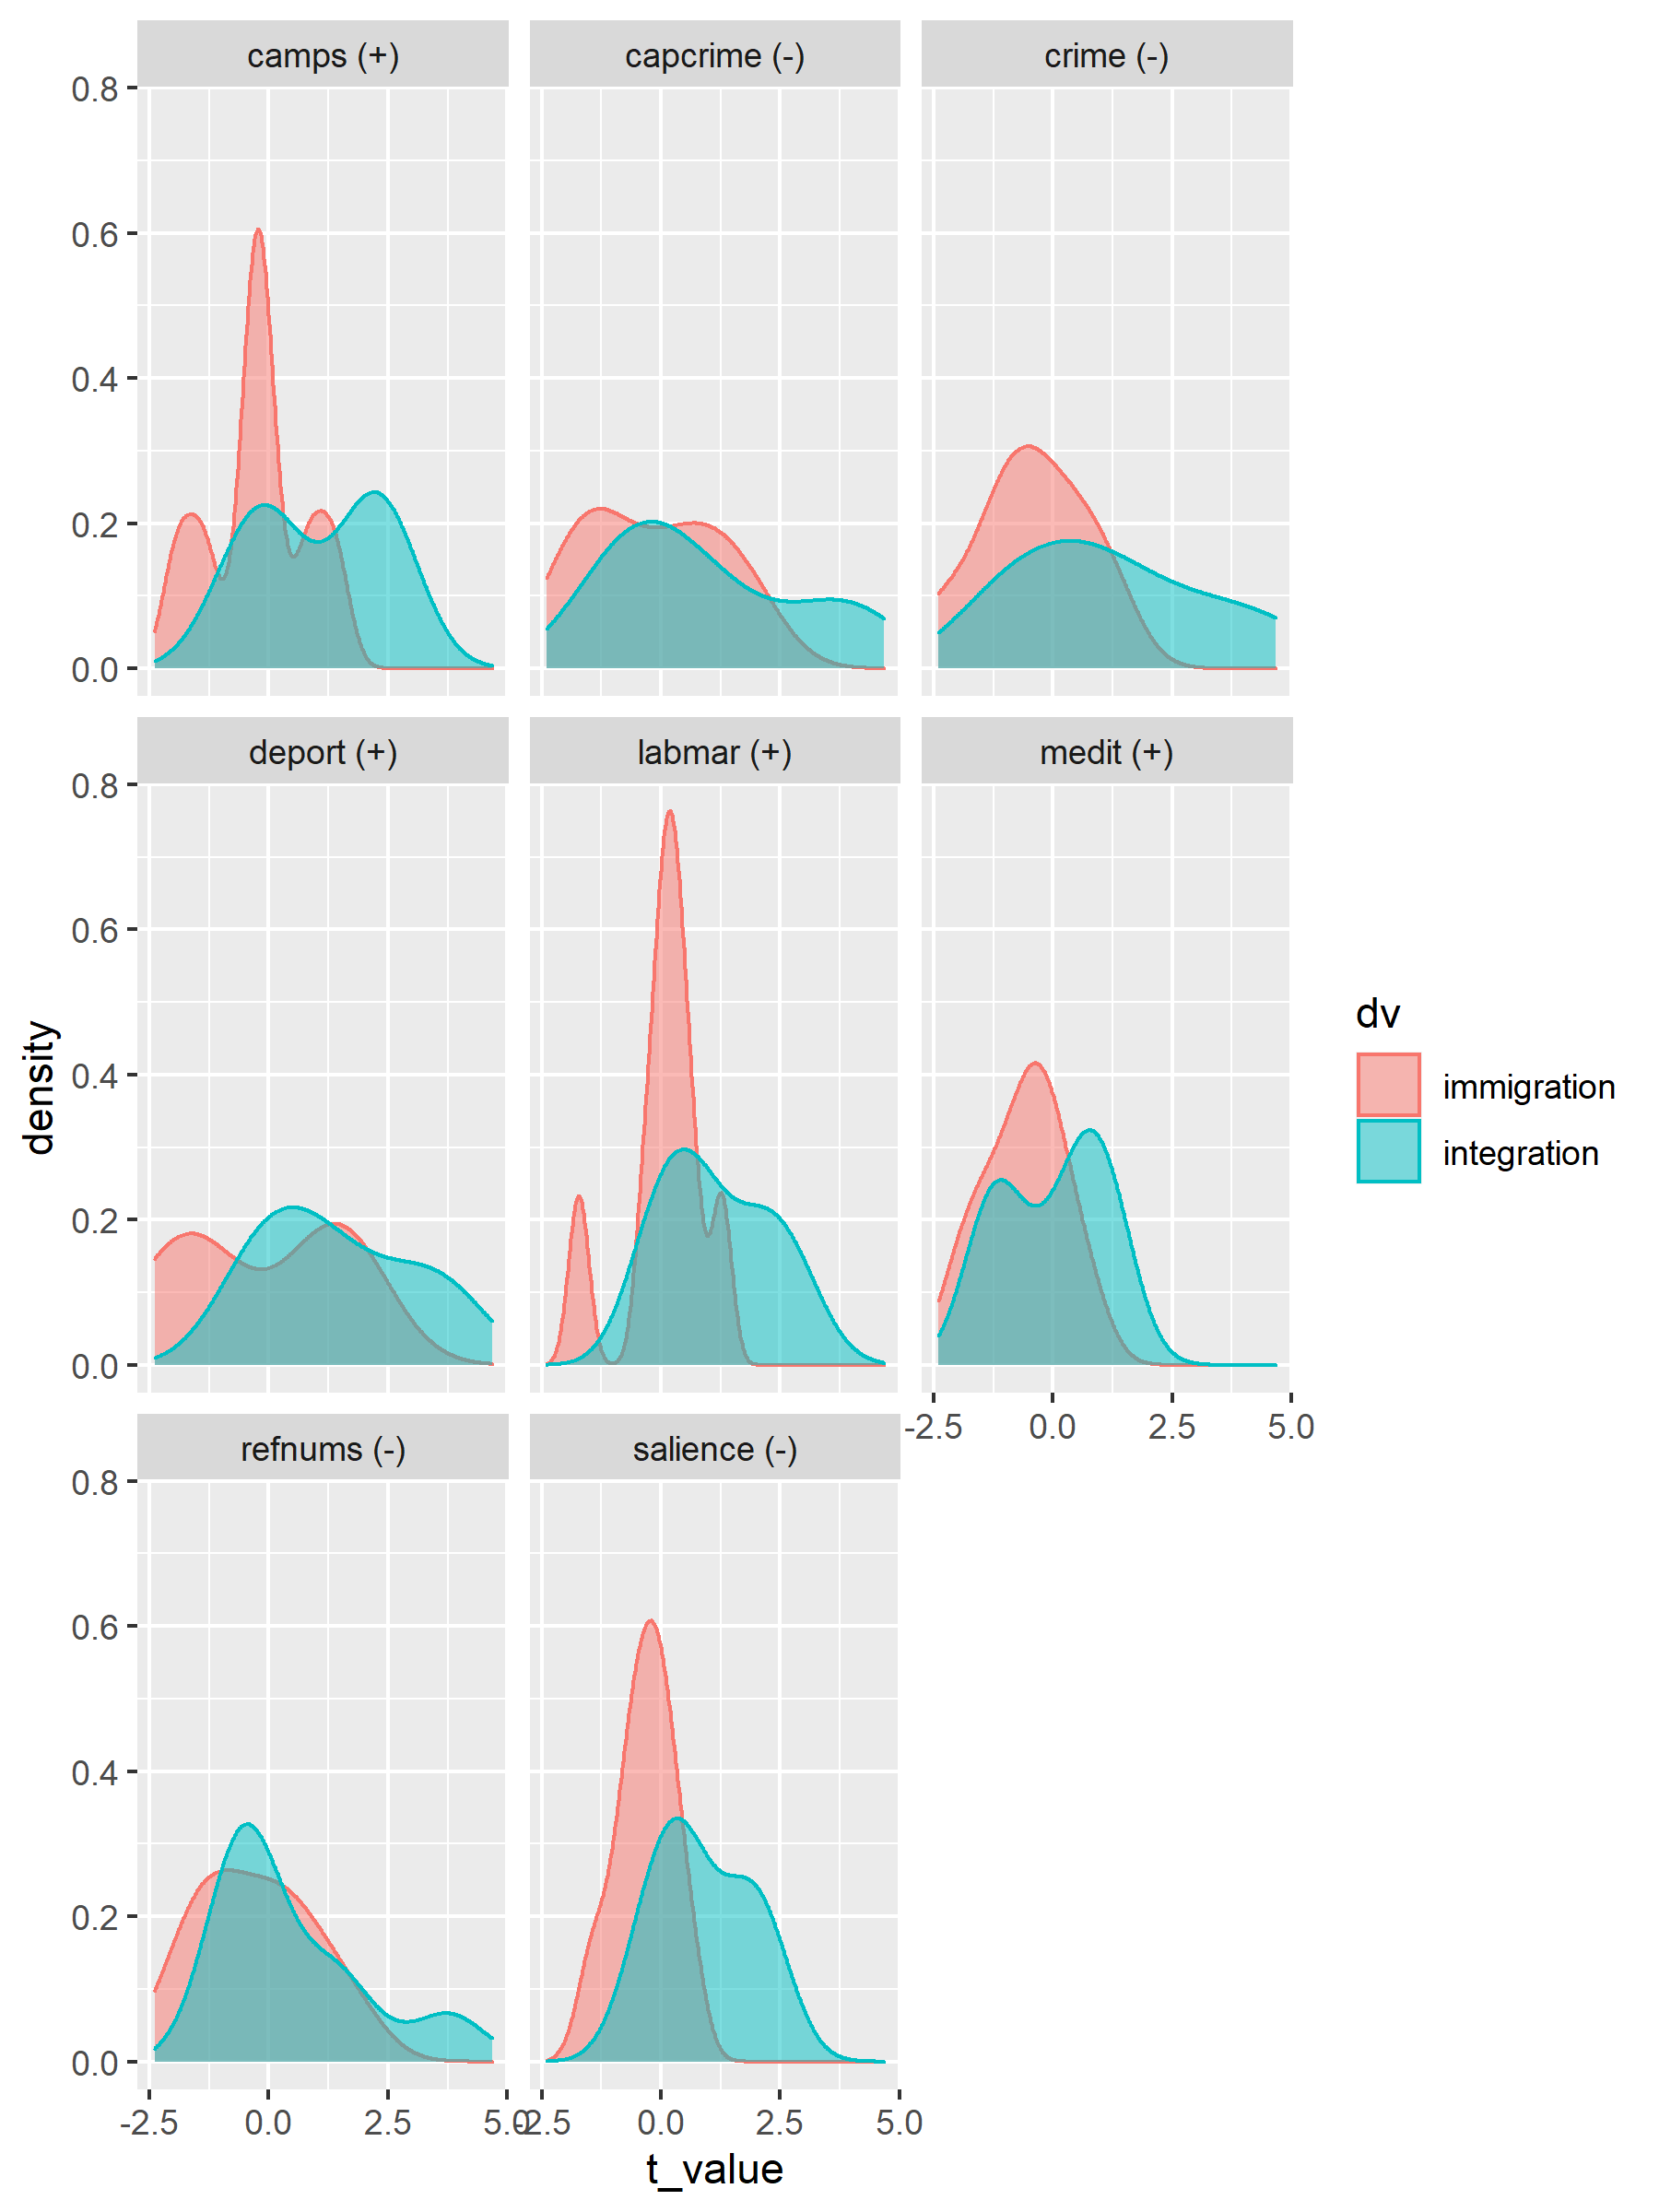
\includegraphics[width = \textwidth]{paper/vis/t_values_noimp.png}
    \caption{Caption}
    \label{fig:t_values}
\end{figure}

\end{document}